\subsection{評価結果}

各項目について本システムとHoloTourを比較した結果を図\ref{figure:pqresult}に示す.図に関しての説明を以下に示す.

\begin{figure}[h]
\begin{center}
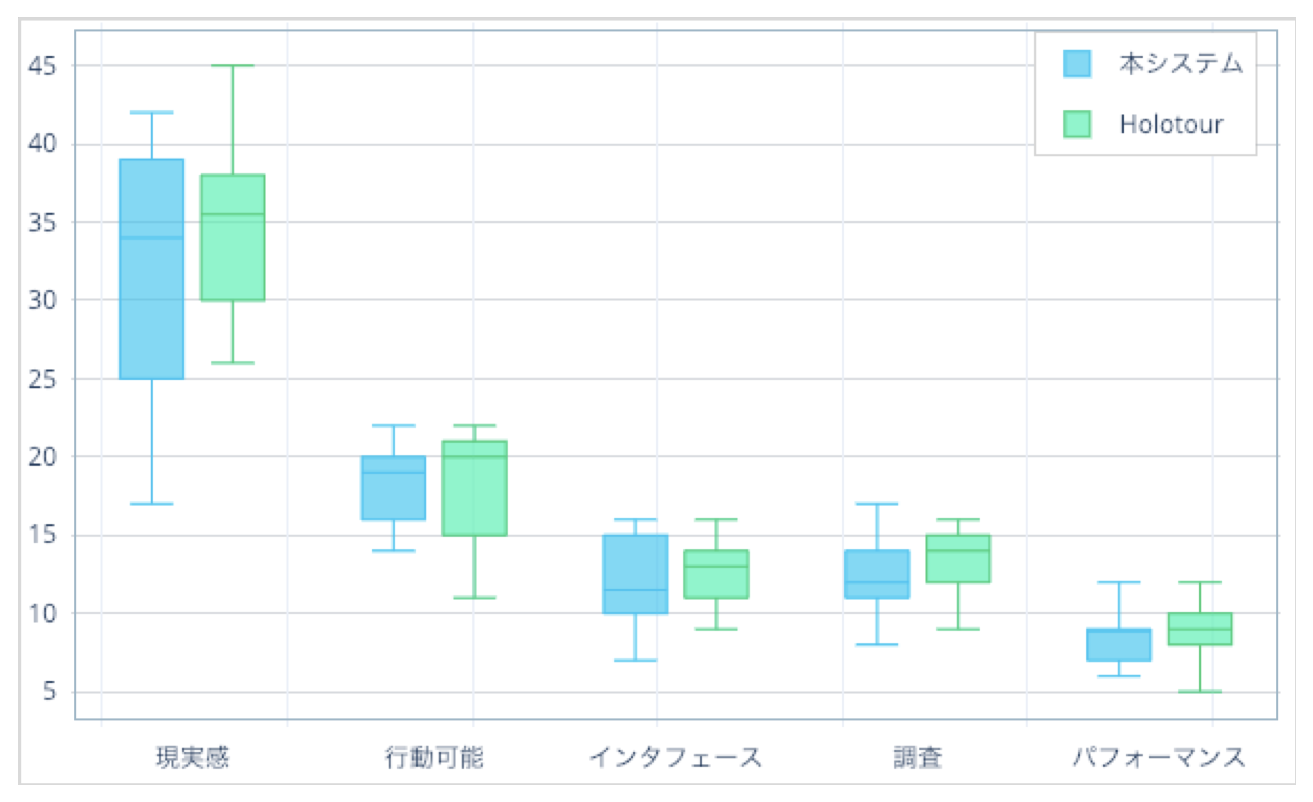
\includegraphics[width=16cm]{img/05_evaluate/result.eps} 
\end{center}
\caption{Presence Questionnaire結果}
\label{figure:pqresult}
\end{figure} 

\subsubsection{現実感}
図\ref{figure:pqresult}ではHoloTourの現実感に関するスコアは最大値,最小値,中央値が本システムよりも高い値となっている.
また2つのシステムの平均スコアを調べたところは本システムが31.8, HoloTourが34.8と平均値がHoloTourの方が高い値となった.
平均値について有意差があるか検定を行った結果, $p$値は0.46であったため本システムとHoloTourの現実感に有意差はみられなかった.

\subsubsection{行動}
%図\ref{figure:pqresult}では
HoloTourの行動に関するスコアは中央値が本システムよりも高い値となっている.しかし,最小値は本システムの方がHoloTourよりも高く,値の差は中央値の差よりも大きい.また最大値は両システムともスコアが22と差はみられなかった.平均を比較すると本システムの平均は18.4, HoloTourは18.0と僅かに本システムの方が高かった.検定を行った結果, $p$値は0.78と有意差はみられなかった.

\subsubsection{インタフェース}
%図\ref{figure:pqresult}では
インタフェースに関してスコアの最大値は本システムとHoloTourで差はみられなかった.しかし,中央値,最小値はHoloTourが本システムよりも高かった.平均を比較すると本システムの平均は12.1, HoloTourは12.7と僅かに本システムの方が低い結果となった.検定を行った結果, $p$値は0.39とこの項目も有意差はみられなかった.

\subsubsection{調査}
%図\ref{figure:pqresult}では
調査に関するスコアの最大値はHoloTourに比べ本システムの方が高かったが,中央値,最小値はHoloTourが本システムよりも高かった.平均を比較すると本システムの平均は12.4, HoloTourは13.6と僅かに本システムの方が低い結果となった.検定を行った結果, $p$値は0.27とこの項目も有意差はみられなかった.

\subsubsection{パフォーマンス}
図\ref{figure:pqresult}ではパフォーマンスに関するスコアの最大値,中央値は同じ値であったが,最小値はHoloTourが本システムよりも高かった.平均を比較すると本システムの平均は8.5, HoloTourは8.9と僅かに本システムの方が低い結果となった.検定を行った結果, $p$値は0.71と有意差はみられなかった.

\subsubsection{ITQとの関係}
図\ref{figure:ITQresult}はPQの各項目の値を縦軸, ITQの値を横軸にとったグラフである.丸い点は本システムのスコアを示しており,菱形の点はHoloTourのスコアを示している.
縦軸方向に青い点と緑の点が離れている時2つのシステムのスコアの差が大きいことがわかる.

\begin{figure*}[t]
\begin{center}
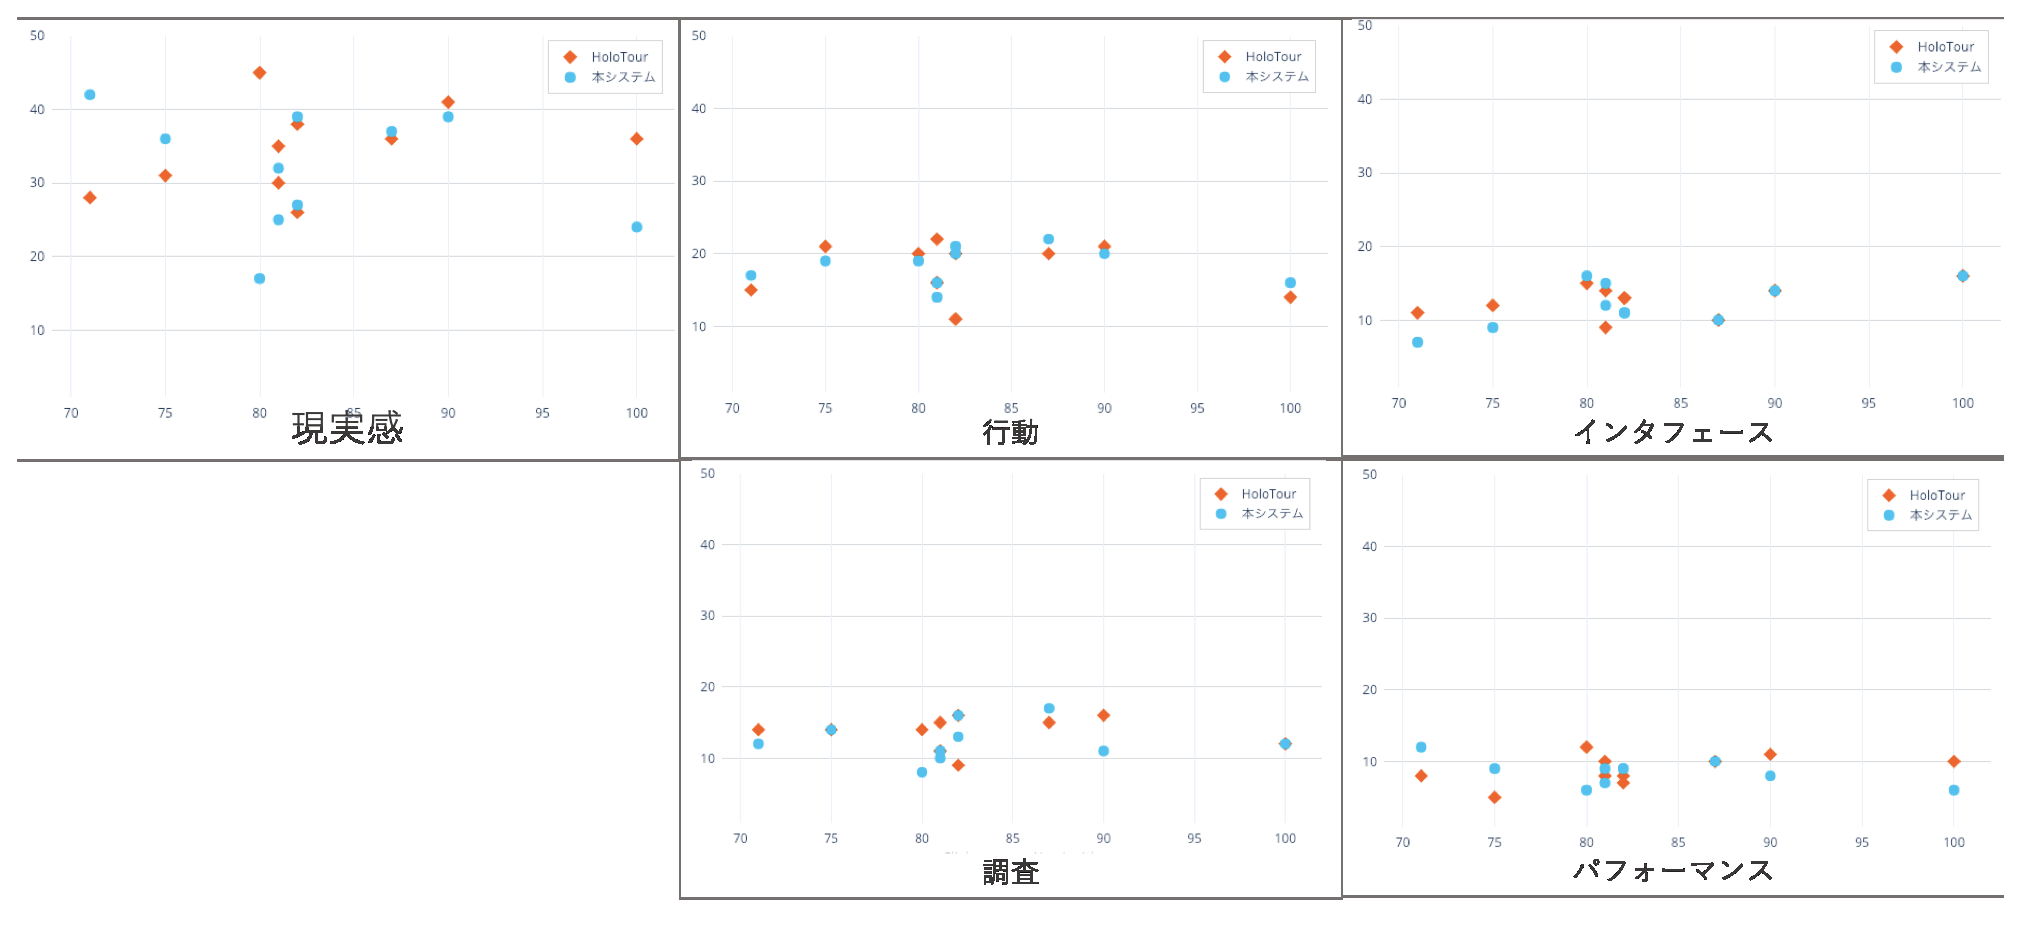
\includegraphics[width=17cm]{img/05_evaluate/ITQresult.eps} 
\end{center}
\caption{PQとITQの関係}
\label{figure:ITQresult}
\end{figure*} 

図\ref{figure:ITQresult}から行動,インタフェース,調査,パフォーマンスのスコアは本システムとHoloTourの間でITQのスコアによる違いはほとんどないことがわかる.しかし現実感に関してITQのスコアが低い被験者ほど本システムを使用した時の方が現実感を高く感じていることがわかる.
逆にITQのスコアが高い人は,本システムよりHoloTourを使用した時により高い現実感を感じている.
本システムよりHoloTourで感じる現実感に高かった被験者はHoloTourのよかったところとして風景が動画で動いているところに現実感を感じていた.逆に本システムの方が現実感があると感じていた被験者に本システムのよかったところを質問したところ,実際に歩くことができることに現実感を感じていた.
\subsubsection{システムについての意見}
被験者に本システムの良いところ,改善してほしいところを質問した.
本システムのよかったところとして遠隔地にいるユーザのアバターに対し親近感を覚えるところや,実際に歩くことができるため没入感が高いとの意見があった.
改善してほしい点として,システムを使用中に音の情報がないことが遠隔地で行動する時の楽しさを減少させているとの意見があった.また風景の更新が遅いことが,実際に遠隔地を歩いている感覚を損ねているとの意見もあった.
\clearpage
\subsubsection{考察}
本システムとHoloTourを比較した時, ITQの値が高い人はHoloTourを使用した際に感じる現実感が高かった.アンケートの回答により表示された風景が動画で出力されていたのが現実感を高める理由であった.そのため没入感を感じやすい人は身体動作よりも視覚情報によって現実感を感じやすいためと考えられる.逆にITQの値が低い人は,視覚情報より身体動作によって現実感を感じるため, HoloTourより本システムを使用した方がより現実感を感じることができたと考えられる.

本システムのよかったところを質問したところ実際に歩くことができる点をあげた人が多かったため,移動を伴う環境でのテレイグジスタンスが現実感を高めるのに有効であると考えられる.
またシステム開発当初は実際の風景と見える 風景が異なるために危険性が懸念されたが,結果的にどの 被験者達からも問題視する声は無かった.これは道路部分を切り抜いた事で現実世界の一部を視認する事ができる事に加えMRによるアプローチが風景表示用球体オブジェクト内の物体も視認できる事が衝突の危険を抑制したためと考えられる.更に本システムで使用したHololensの視野角は35度程度であるため,現実の環境を認識しやすかったことも理由の1つと考えられる.本問題は重要なので今後より精密に評価を行う予定である.

さらにシステムの改善してほしいところを質問したところ,音がなく寂しいところや風景の更新がスムーズに行われないところをあげるユーザが多かった.我々は音をHololensの内蔵スピーカーによるガイドや他ユーザの声の出力,風景更新時のサーバとの通信回数削減によりこれらの問題を解決する.
